\chapter{モジュール情報及び品質試験結果管理システム}
前章で述べたように、モジュール生産及び品質試験を世界中で行う。
これらの情報はデータベースシステムを用いて管理することが決まっていて、現在この開発を行っている。
システムについては、大きく2つに分けられる。
チェコに設置し、試験運用をしている中央データベースと、各組み立て期間に設置し、運用の際に使用するローカルデータベースである。
本章ではこれらのデータベースについて説明する。また、システム開発の中で私が開発を行った仕組みや機能について詳細に説明する。

\section{中央データベース}
\subsection{中央データベースの概要}
\subsubsection{概要}
中央データベースは、新型内部飛跡検出器の製造に関する全ての情報の保存を目的として開発されたデータベースである。
ユニコーン大学が開発、運用を行っていて、チェコにデータベースサーバーが設けられている。
新型内部飛跡検出器は、前述したようにピクセル検出機とストリップ検出機にから構成される。
これらを生産するにあたって、シリコンセンサーや電気基板といった小さな部品から製造を行い、それらを用いたモジュールの組み立て、複数モジュールを搭載したstaveやringの組み立てを経て検出器が完成する。
また各組み立て段階において、動作確認等を目的とした品質試験を行う。
これらの過程における全ての構成部品の情報、及び品質試験結果を中央データベースに保存する。

\subsubsection{意義}
中央データベースに保存された情報は、検出器運転時の参考値として扱われる。
モジュールを例にだすと、品質試験で読み出し試験を行った際の最適な設定値を中央データベースに保存するため、実際の運転時に参照することができる。
また運転前の状態における検出器の性能、運転前後での検出機性能比較を行うことができる。
HL-LHCでは1章で述べたように、運転時における放射線量が大きいものとなるため、運転前後での放射線損傷の影響の研究を行うことができ、検出機の寿命の推定や放射線損傷に関しての対策に役に立てることができる。

それらしいデータかこんな解析に役立てたいみたいなのを考え中です。

\subsection{モジュール情報構造および構成部品との関係の実装}
中央データベースにモジュールを登録するためには、1章で述べたようにモジュールの種類、モジュールを構成する部品といった情報構造を決定し、データベース上に定義しておく必要がある。この情報構造をデータベースに実装し、登録できる仕組みを整えた。
詳細な種類と構造については表\ref{pd_module_structure}に示す。
またある種類に関する例を図\ref{example_module_structure}に示す。

\begin{table}[tbp]
\begin{center}
\caption[中央データベースにおけるモジュールの種類と構造]{中央データベースにおけるモジュールの種類と構造}
\label{pd_module_structure}
  \begin{tabular}{|ll|} \hline
    種類 & 構成する部品(数) \\ \hline
    Triplet L0 stave module   &  Single bare module(3) \\
                              &  Triplet stave PCB(1) \\\hline
    Triplet L0 Ring0 module   &  Single bare module(3) \\
                              &  Triplet R0 PCB(1) \\\hline
    Triplet L0 Ring0.5 module &  Single bare module(3) \\
                              &  Triplet R0.5 PCB(1) \\\hline
    L1 quad module            &  Quad bare module(1) \\
                              &  Quad PCB(1) \\\hline
    Outer system quad moudle  &  Quad bare module(1) \\
                              &  Quad PCB(1) \\\hline
    Outer system quad moudle  &  Dual bare module(1) \\
                              &  Dual PCB(1) \\\hline
    Digital triplet L0 stave module   &  Digital single bare module(3) \\
                                      &  Triplet stave PCB(1) \\\hline
    Digital triplet L0 Ring0 module   &  Digital single bare module(3) \\
                                      &  Triplet R0 PCB(1) \\\hline
    Digital triplet L0 Ring0.5 module &  Digital single bare module(3) \\
                                      &  Triplet R0.5 PCB(1) \\\hline
    Digital quad module       &  Digital quad bare module(1) \\
                              &  Quad PCB(1) \\\hline
    Digital L1 quad moudle    &  Digital quad bare module(1) \\
                              &  Quad PCB(1) \\\hline
    Dummy triplet L0 stave module   &  Dummy single bare module(3) \\
                                    &  Triplet stave PCB(1) \\\hline
    Dummy triplet L0 Ring0 module   &  Dummy single bare module(3) \\
                                    &  Triplet R0 PCB(1) \\\hline
    Dummy triplet L0 Ring0.5 module &  Dummy single bare module(3) \\
                                    &  Triplet R0.5 PCB(1) \\\hline
    Dummy quad module       &  Dummy quad bare module(1) \\
                            &  Quad PCB(1) \\\hline
    Dummy L1 quad moudle    &  Dummyl quad bare module(1) \\
                            &  Quad PCB(1) \\ \hline
  \end{tabular}
\end{center}
\end{table}

\begin{figure}[bpt]\centering
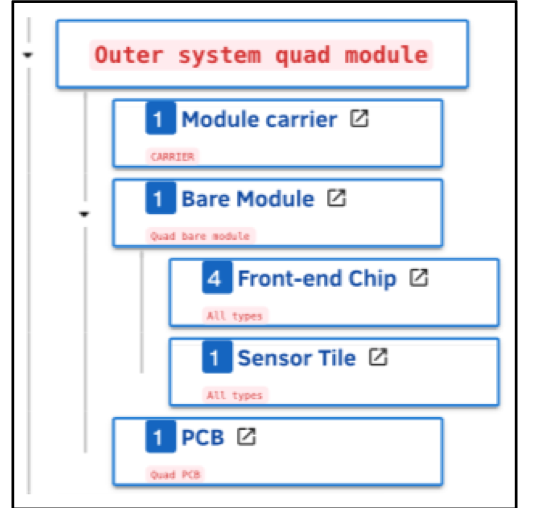
\includegraphics[width=7cm]{example_module_structure}
\caption[モジュール構造の一例]{モジュール構造の一例}
\label{example_module_structure}
\end{figure}

\subsection{組み立て工程および品質試験の情報形式の実装}
モジュールの情報構造の実装に加えて、品質試験の情報を正確に管理するには、モジュール組み立て工程の情報と付随する品質試験の項目をデータベース上に定義する必要がある。これを実装し、テスト結果を適切な組み立て工程へアップロードできる仕組みを整えた。

詳細な構造を図\ref{pd_stage_structure}に示す。

\begin{table}[tbp]
\begin{center}
\caption[中央データベースにおける組み立て工程と付随するテスト項目]{中央データベースにおける組み立て工程と付随するテスト項目}
\label{pd_stage_structure}
  \begin{tabular}{|ll|} \hline
    組み立て項目 & 付随する組み立て情報及び品質試験項目 \\ \hline
    1. Bare to PCB assembly & Visual Inspection \\ 
                            & Metrology \\
                            & Mass measurement \\
                            & Glue information \\\hline
    2. Wirebonding          & Visual Inspection \\ 
                            & Wirebond information \\
                            & (Wirebond pull test)\\
                            & First power up\\
                            & Sensor IV\\
                            & SLDO VI\\
                            & Chip configuration\\
                            & Pixel failure test\\\hline

    3. Wirebond Protection  & Visual Inspection \\ 
                            & Potting information \\
                            & Sensor IV \\
                            & Chip configuration\\
                            & Readout for basic electrical \\\hline

    4. Parylene Coating     & Visual Inspection \\ 
                            & Palylene information \\
                            & Mass measurement \\
                            & Sensor IV \\
                            & Chip configuration\\
                            & Readout for basic electrical \\
                            & Bump bond quality \\\hline

    5. Thermal Cycling      & Visual Inspection \\ 
                            & Thermal cycling info \\
                            & Sensor IV \\
                            & Chip configuration\\
                            & Readout for basic electrical \\\hline

    6. Burn-in              & Visual Inspection \\ 
                            & Metrology \\
                            & Mass Measurement \\
                            & First power up\\
                            & Sensor IV\\
                            & SLDO VI\\
                            & Chip configuration\\
                            & Pixel failure test\\\hline

    7. Reception            & \\\hline 
  \end{tabular}
\end{center}
\end{table}

\newpage

\section{ローカルデータベース}
\subsection{ローカルデータベースの概要と意義}
中央データベースでは、前述したようにモジュールの情報のみならず新型内部飛跡検出器に関わるすべての情報を管理する。データベースの機能としては汎用的に使えるようなものになっている。
モジュールの組み立て及びその品質試験に関しては3章で述べたように工程が複数に渡り、行う品質試験の数も多い。1つの生産現場で多いところでは数千個のモジュールを作ることになるため、データ管理が簡単にかつ円滑に進むようになっているのが好ましい。
このような理由から、生産現場での生産性、利便性に特化し、円滑な生産をサポートすることを目的としたデータベースシステム(ローカルデータベース)を開発している。
システムの概要図を図\ref{localdb_overview}に示す。オープンソースのサービスであるMongoDBを各生産現場で使い、開発したウェブアプリケーションを併用することでデータ管理や中央データベースとのデータ同期を行うシステムとなっている。

\begin{figure}[bpt]\centering
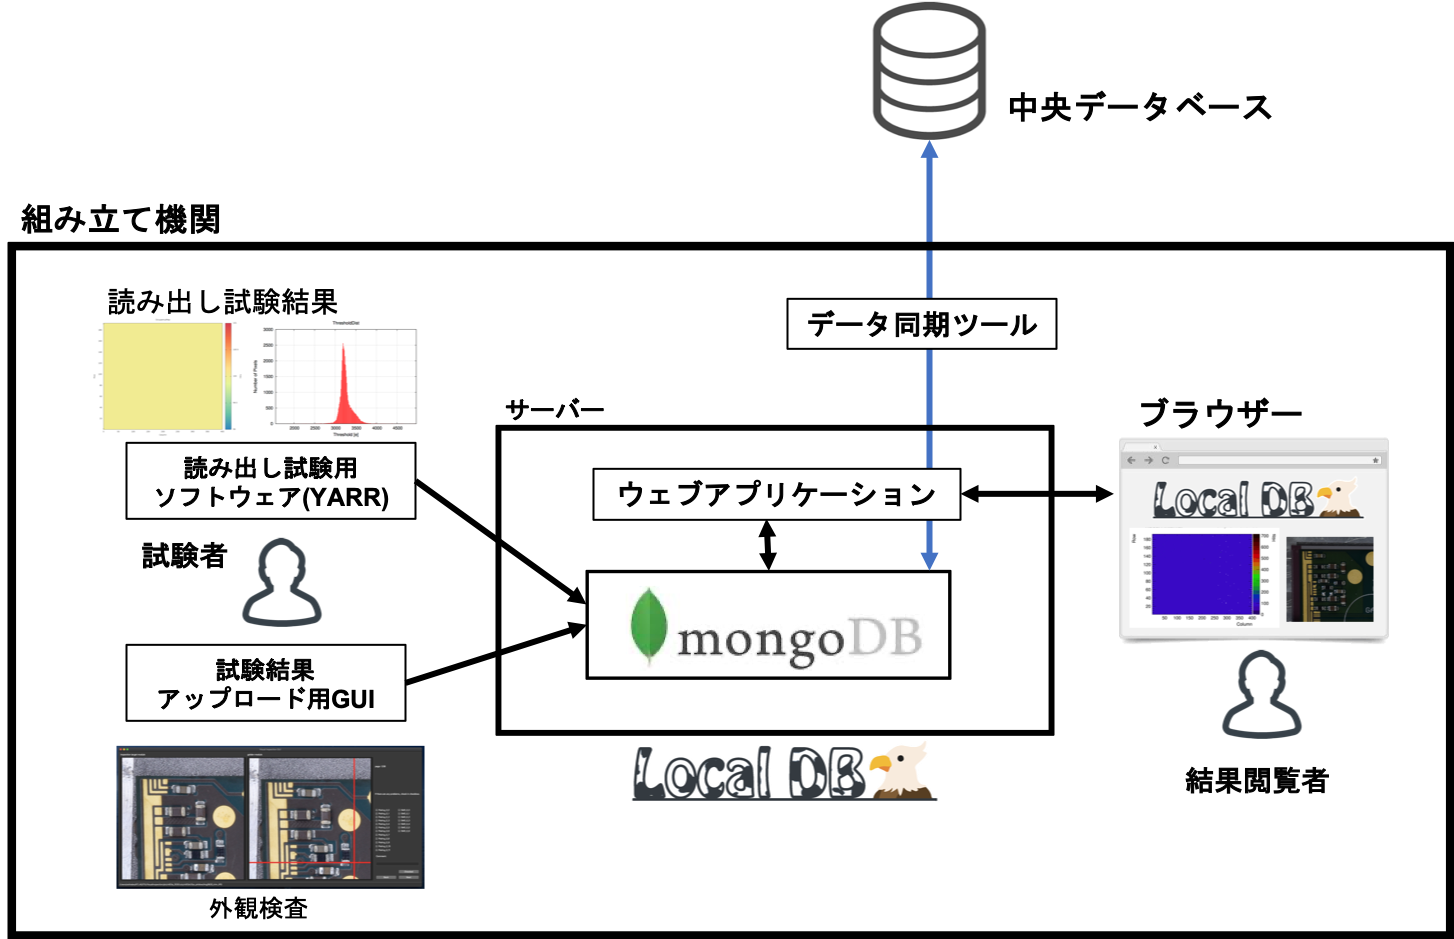
\includegraphics[width=15cm]{localdb_overview}
\caption[ローカルデータベースシステムの概要]{ローカルデータベースシステムの概要}
\label{localdb_overview}
\end{figure}

具体的にローカルデータベースは以下のような利点を持つ。

\begin{itemize}
  \item ローカルにデータベースサーバーを立てるためアクセス速度が早く、円滑にデータ管理を行うことができる。
  \item モジュールの組み立て工程を管理し、生産者の適切な処理を助ける。
  \item モジュールに特化したデータ管理、解析を行うことで異常をいち早く検知できる。
  \item 試験者の情報や試験時間など、テスト結果以外の必要な情報を正確に管理できる。
\end{itemize}

\subsection{開発状況と今後の方針}
現在、以下のような機能を実装している。

今後は他の試験についても機能を拡張していきたい。

\subsection{チュートリアルと普及状況}
ローカルデータベースの機能の普及を目的として、2020年2月にCERN研究所にてシステムのチュートリアルを行った。
このチュートリアルは以下のような2つのセッションに分けて行った。

\begin{itemize}
  \item 参加者が実際にサーバーの設定、各ソフトウェアのインストールを行いながら機能を実践するセッション(2月3日から6日まで)
  \item 私が参加者の前で実際に機能を実践し、システムや使い方に対して議論を行うセッション(2月7日)
\end{itemize}

それぞれのセッションの様子を図\ref{Tutorial_picture}に示す。
数多くの議論を行い、有益なフィードバックを得ることができた。

\begin{figure}[bpt]
  \begin{center}
  \begin{minipage}{0.4\hsize}
    
\includegraphics[width=10mm]{figure}
  \end{minipage}
  \begin{minipage}{0.4\hsize}
    
\includegraphics[width=10mm]{figure}
  \end{minipage}
  \caption[ハンズオンとハンズオフ]{ハンズオンとハンズオフ}
  \label{Tutorial_picture}
  \end{center}
\end{figure}

これを経て現在ローカルデータベースは世界10箇所にて導入され、試験運用が開始している。
また将来的には全組み立て機関で使うことが決定しており、それに向けたシステム開発、サポートが必要となっている状況である。
ローカルデータベースについて、試験運用を行っている機関を表\ref{localdb_world_site}、世界地図を\ref{localdb_world_map}に示す。

\begin{table}[tbp]
\begin{center}
\caption[ローカルデータベース運用期間]{ローカルデータベース運用期間}
\label{localdb_world_site}
  \begin{tabular}{|ll|} \hline
    1 & 2 \\ \hline
    result 1 & result 2 \\ \hline 
  \end{tabular}
\end{center}
\end{table}

\begin{figure}[bpt]\centering
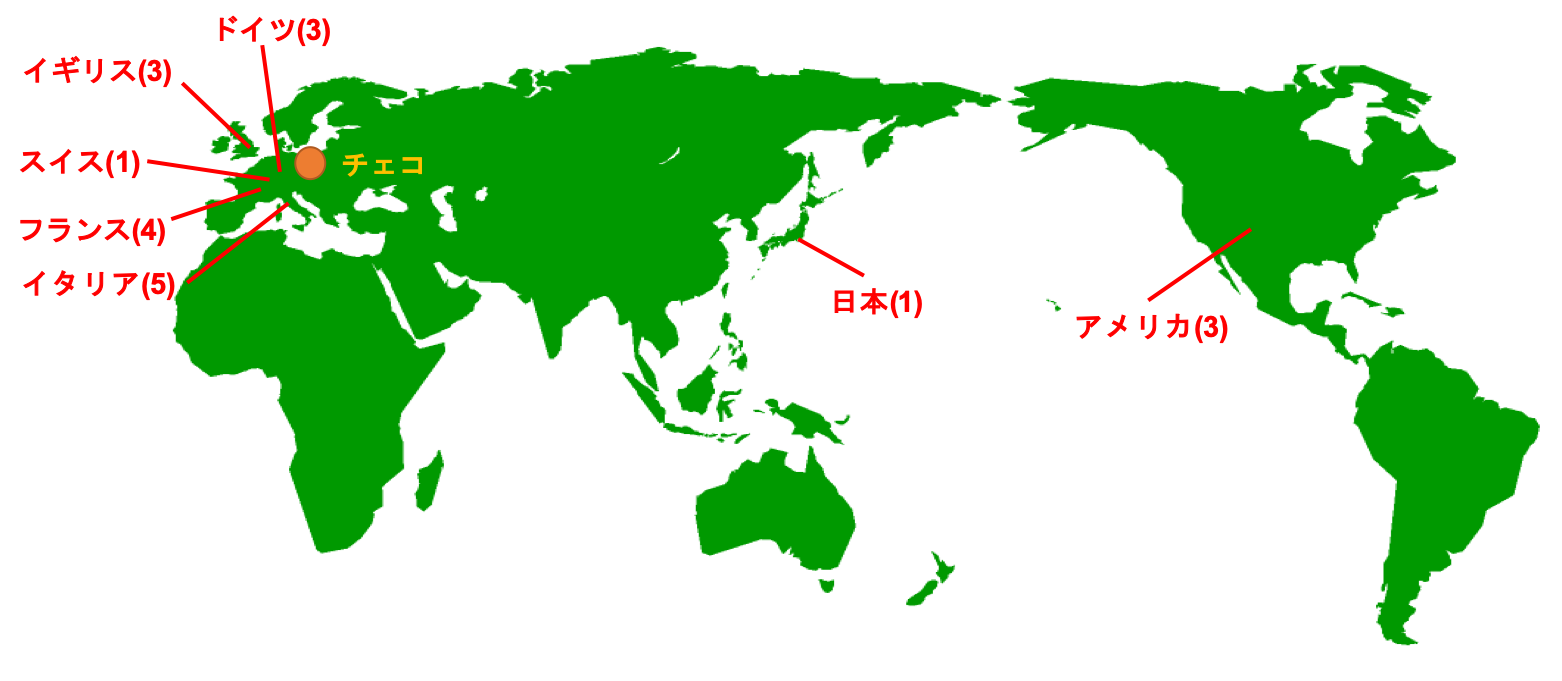
\includegraphics[width=10cm]{localdb_world_map}
\caption[ローカルデータベース地図]{ローカルデータベース地図}
\label{localdb_world_map}
\end{figure}

\subsection{MongoDBとその内部構造}
MongoDBの内部構造について簡単に図\ref{mongodb_schema}に示す。

\begin{figure}[bpt]\centering

\includegraphics[width=1cm]{figure}
\caption[MongoDBの構造]{MongoDBの構造}
\label{mongodb_schema}
\end{figure}

モジュール及び品質試験に関する構造として、図\ref{localdb_mongodb_structure}にまとめた。

\begin{figure}[bpt]\centering

\includegraphics[width=1cm]{figure}
\caption[品質試験周りにおける]{品質試験周りにおける構造}
\label{localdb_mongodb_structure}
\end{figure}

\subsection{中央データベースとの情報同期ツール}
生産時にはローカルデータベースと中央データベースにおいて、情報の同期が必要となる。例えば、モジュールのIDや組み立て工程、テスト結果といった情報があげられる。
この情報同期のためのインターフェースツールを開発した。主に開発した項目については以下の2つである。
\begin{itemize}
  \item モジュールのID及びモジュールを構成するFE chipのIDのダウンロード機能
  \item 品質試験の中の読み出し試験に関しての試験結果アップロード機能
\end{itemize}

ダウンロード機能についての詳細を図\ref{pd_download_info}にまとめた。中央データベースに登録されているモジュールの ID、FE chipのIDとその数、対応関係をダウンロードしてくるものとなる。
\begin{figure}[bpt]\centering

\includegraphics[width=1cm]{figure}
\caption[ダウンロード機能の概要]{ダウンロード機能の概要}
\label{pd_download_info}
\end{figure}

アップロード機能についての詳細を図\ref{pd_upload_info}にまとめた。YARRで取得されるデータはFE chipごとであるため、取得ファイルはFE chipごとにアップロードすることとしている。

\begin{figure}[bpt]\centering

\includegraphics[width=1cm]{figure}
\caption[アップロード機能の概要]{アップロード機能の概要}
\label{pd_upload_info}
\end{figure}

生産の際には、これら機能は後述するウェブアプリケーションを通して使用する。具体的な使用方法については、後の節で述べる。処理速度に関する性能評価を6章で述べる。

\subsection{情報管理アプリケーション}
\subsubsection{概要、意義}
各組み立て機関において、試験者が品質試験結果を閲覧、管理するツールとして、ウェブアプリケーションを開発した。
試験結果を迅速に分かりやすく見るシステムを作り、円滑な生産の補助や異常結果の早期発見を目的としている。
アプリケーションの機能として、具体的に以下のような項目を実装している。

\begin{itemize}
  \item 登録モジュール及び品質試験結果の情報閲覧機能
  \item 登録モジュール及び品質試験結果の検索機能
  \item 試験者情報の管理及び各種機能
  \item 中央データベースへアップロードする品質試験結果の登録と組み立て工程の管理機能
  \item 中央データベースとのデータ同期機能
\end{itemize}

それぞれの機能の詳細を以下に記す。

\subsubsection{登録モジュール及び品質試験結果の情報閲覧}
アプリケーションを用いて、登録したモジュール情報やアップロードした品質試験結果を閲覧することができる。
モジュールページの例を図\ref{webapp_modulepage}に、読み出し試験の結果ページの例を図\ref{webapp_scanpage}に示す。

\begin{figure}[bpt]\centering

\includegraphics[width=1cm]{figure}
\caption[モジュールページの例]{モジュールページの例}
\label{webapp_modulepage}
\end{figure}

\begin{figure}[bpt]\centering

\includegraphics[width=1cm]{figure}
\caption[読み出し試験結果ページの例]{読み出し試験結果ページの例}
\label{webapp_scanpage}
\end{figure}

\subsubsection{登録モジュール及び品質試験結果の検索機能}
登録モジュールや品質試験結果の一覧ページに検索機能を実装した。
確認したいモジュール情報や試験結果を迅速に取得し、閲覧できることを目的としている。検索機能を使用している様子を図\ref{webapp_search_function}に示す。
一般的なウェブページの検索エンジンのように扱うことができる。

\begin{figure}[bpt]\centering

\includegraphics[width=1cm]{figure}
\caption[検索機能の様子]{検索機能の様子}
\label{webapp_search_function}
\end{figure}

また生産に向けて、検索にかかる処理速度測定を行った。これについては付録Aで詳細を述べる。

\subsubsection{試験者情報の管理及び各種機能}

異常があった際に確認することを目的として、誰が試験を行ったかを記録することが必要である。
また、モジュールの登録や中央データベースとのデータ同期など、データベースの機能使用を制限することも必要である。
これらを目的として、試験者及びデータベース使用者情報の管理システムを開発、実装した。
この機能の概要について図?に示す。
データベースの管理者が試験者を登録することができる。また以下のような機能が登録試験者に制限される。

\begin{itemize}
  \item 試験結果のアップロード
  \item 中央データベースへアップロードする品質試験結果の登録と組み立て工程の管理機能
  \item 中央データベースとのデータ同期機能
\end{itemize}

上記の他に、登録ユーザは結果に対するコメント機能、任意のタグを貼る機能を使用することができる。各種機能について、使用したときの様子を図\ref{webapp_comment}、\ref{webapp_tag}に示す。

\begin{figure}[bpt]\centering

\includegraphics[width=1cm]{figure}
\caption[コメント機能]{コメント機能}
\label{webapp_comment}
\end{figure}

\begin{figure}[bpt]\centering

\includegraphics[width=1cm]{figure}
\caption[タグ機能]{タグ機能}
\label{webapp_tag}
\end{figure}

\subsubsection{中央データベースへアップロードする品質試験結果の登録と組み立て工程の自動更新}
ローカルデータベースへアップロードした品質試験結果の中から、本結果として中央データベースへアップロードする結果を選択する機能を開発した。
品質試験は3章で述べたように、各モジュール、各組み立て工程に対して行うものであるため、結果選択も同様に工程毎に行うことを想定している。
結果選択後、データベースにおける組み立て工程の情報も次のものへ自動的に更新する機能となっている。

あるモジュール、組み立て工程に対して結果を選択する様子を図\ref{webapp_sign_off}に示す。組み立て工程も自動更新されていることがわかる。

\begin{figure}[bpt]\centering

\includegraphics[width=1cm]{figure}
\caption[サインオフ機能]{サインオフ機能}
\label{webapp_sign_off}
\end{figure}

\subsubsection{中央データベースとのデータ同期機能}
モジュールのダウンロード機能、読み出し試験結果のアップロード機能をアプリケーションの中で使うことができる仕組みを実装した。
モジュールのトップページからこの操作が可能となっている。

\section{量産時の情報登録・データ同期の流れ}
想定している、モジュールに関しての組み立て工程とデータベースシステムでのユーザ操作の流れを図\ref{dbsystem_flow}に示す。

\begin{figure}[bpt]\centering

\includegraphics[width=1cm]{figure}
\caption[データベースシステム操作の流れ]{データベースシステム操作の流れ}
\label{webapp_sign_off}
\end{figure}

各ユーザ操作は上述したウェブアプリケーションを用いて行う。
最終的には、モジュールの情報及び選択した品質試験の結果が全て中央データベースへ同期されている状態となる。
この流れのデモンストレーションを、学内のプロトタイプモジュールを用いて行った。詳細を5章で述べる。

\section{モジュール生産状況の解析}
上述したデータベースシステムを使って、将来的には世界でモジュール生産がどれだけ進んでいるのかを解析する機能を作ることを考えている。
全てのモジュールの状況は各生産場所のローカルデータベース上に記録され、組み立て工程ごとに中央データベースへデータ同期する。
そのため生産時には、中央データベースで全てのモジュールに関して、現在の組み立て情報を取得できることができ、世界的な生産状況の解析を行うことができる。
想定している解析結果のイメージ図を図\ref{production_analysis}に示す。

\begin{figure}[bpt]\centering

\includegraphics[width=1cm]{figure}
\caption[生産時のモジュール組み立て状況解析の例]{生産時のモジュール組み立て状況解析の例}
\label{production_analysis}
\end{figure}

